\documentclass[tikz, border=2pt]{standalone}
\usepackage{amsmath}
\usetikzlibrary{calc, decorations.markings, positioning}

\begin{document}
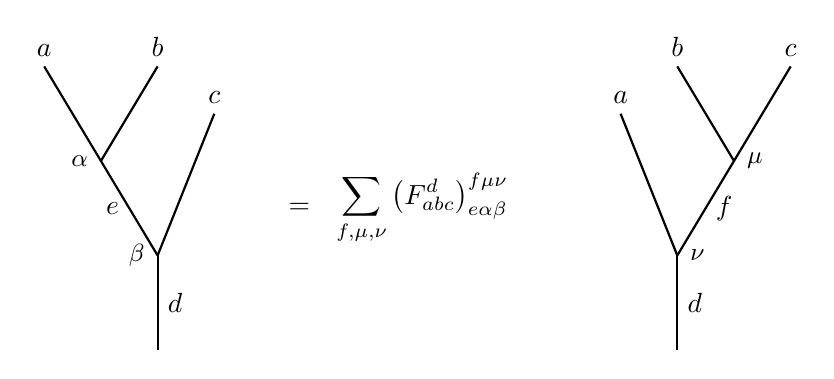
\begin{tikzpicture}[thick, scale=1.2, baseline=(current bounding box.center)]
    % Define style for lines
    \tikzset{anyon/.style={postaction={decorate}, decoration={markings, mark=at position 0.55 with {\arrow{>}}}}}
    
    % LEFT TREE: ((a b)_e c)_d
    \begin{scope}[shift={(0,0)}]
        % Coordinates
        \coordinate (root) at (0,0);
        \coordinate (v_beta) at (0,1);
        \coordinate (v_alpha) at (-0.6, 2);
        \coordinate (top_c) at (0.6, 2.5); % Endpoint for c
        \coordinate (top_a) at (-1.2, 3); % Endpoint for a
        \coordinate (top_b) at (0, 3);    % Endpoint for b
        
        % Lines
        \draw (root) -- (v_beta) node[midway, right] {$d$};
        \draw (v_beta) -- (top_c) node[above] {$c$};
        \draw (v_beta) -- (v_alpha) node[midway, left] {$e$};
        \draw (v_alpha) -- (top_a) node[above] {$a$};
        \draw (v_alpha) -- (top_b) node[above] {$b$};
        
        % Vertex Labels (Indices)
        \node[left=1pt] at (v_beta) {\small $\beta$};
        \node[left=1pt] at (v_alpha) {\small $\alpha$};
    \end{scope}
    
    % EQUALS SIGN
    \node at (1.5, 1.5) {$=$};
    \node at (2.8, 1.5) {$\displaystyle \sum_{f, \mu, \nu} \left(F_{abc}^d\right)_{e \alpha \beta}^{f \mu \nu}$};
    
    % RIGHT TREE: (a (b c)_f)_d
    \begin{scope}[shift={(5.5,0)}]
        % Coordinates
        \coordinate (root) at (0,0);
        \coordinate (v_nu) at (0,1);
        \coordinate (v_mu) at (0.6, 2);
        \coordinate (top_a) at (-0.6, 2.5); % Endpoint for a
        \coordinate (top_b) at (0, 3);      % Endpoint for b
        \coordinate (top_c) at (1.2, 3);    % Endpoint for c
        
        % Lines
        \draw (root) -- (v_nu) node[midway, right] {$d$};
        \draw (v_nu) -- (top_a) node[above] {$a$};
        \draw (v_nu) -- (v_mu) node[midway, right] {$f$};
        \draw (v_mu) -- (top_b) node[above] {$b$};
        \draw (v_mu) -- (top_c) node[above] {$c$};
        
        % Vertex Labels (Indices)
        \node[right=1pt] at (v_nu) {\small $\nu$};
        \node[right=1pt] at (v_mu) {\small $\mu$};
    \end{scope}

\end{tikzpicture}
\end{document}
